\documentclass[11pt]{article}
\usepackage[margin=1in]{geometry}
\usepackage{graphicx}
\usepackage{hyperref}
\usepackage{booktabs}
\usepackage{longtable}
\usepackage{tikz}
\usetikzlibrary{positioning,arrows.meta}

% Inserts a figure from ../figures if it exists (run the pipeline first)
\newcommand{\safefig}[2]{%
  \IfFileExists{../figures/#1.png}{%
    \begin{figure}[htbp]\centering
      \includegraphics[width=0.75\linewidth]{../figures/#1.png}
      \caption{#2}
    \end{figure}}{%
    \textbf{[Missing figure: \detokenize{#1} -- run the pipeline]}\par}}

\title{Trouvaille: AI-Powered Outfit Recommendation\\Deliverable 3 -- Final Deployment \& Technical Report}
\author{Romesha Afzaal (24L-3001) \and Aliza Nadeem (24L-3024)}
\date{}

\begin{document}
\maketitle

\begin{abstract}
Online outfit shopping in Pakistan is slow and fragmented: shoppers browse many brand sites and
cannot easily search by occasion, budget, skin undertone or body type. Trouvaille is a web app that
recommends outfits from eight Pakistani clothing brands. We scraped and cleaned about 25,000 products,
embedded their text with a pretrained sentence encoder \cite{reimers2019sbert,wang2020minilm}, and trained
a PyTorch MLP \cite{paszke2019pytorch} to predict which occasions each product suits. On a held-out test set the model reaches
a macro F1 of 0.928 and an AUC-ROC of 0.980, and a subgroup analysis shows weaker performance on some brands and categories.
The model is deployed in a Streamlit app with free-text occasion matching and budget, color, size, undertone and body-type filters.
Occasion labels and the undertone and body-type filters are rule-based heuristics, which we document as limitations.
\end{abstract}

\section{Phase 1: Problem Definition}

\subsection{Problem Statement}
Online fashion shopping is time-consuming and fragmented. A shopper preparing for an event, such as a wedding, concert, presentation or office day, must search for each clothing item separately, keep a budget in mind, and guess whether the pieces will look good together. Existing platforms rely on keyword search and category filters, which work poorly for requests like ``a black outfit under Rs.\ 15,000 for a concert'', because this single sentence combines colour, budget, occasion and multiple garments.

A second pain point is that most platforms ignore the individual. Recommendations are rarely adjusted for skin tone or body type, so shoppers often receive items that do not suit them, and rely on product ratings alone as a proxy for quality. Finally, no mainstream tool checks whether a complete outfit is appropriate for the type of event. The result is wasted time, over-budget purchases, returns, and low confidence in online buying.

Trouvaille addresses this by letting users describe what they need in plain language and returning a complete, budget-aware, occasion-appropriate outfit built from real products.

\subsection{Target Audience}
The primary users are online shoppers in Pakistan, particularly students and young professionals, who buy clothing for specific events on a limited budget and want quick, confident styling decisions. Secondary users include shoppers who find fashion choices overwhelming, and people who are underserved by generic recommendations because of their body type or skin tone.

From a research perspective, the project targets a gap between existing work: most recommender systems rank single items, whereas Trouvaille combines (i) natural-language query understanding, (ii) inclusive re-ranking by skin tone, body type and ratings, (iii) budget-constrained outfit composition, and (iv) an occasion-appropriateness check, all in one pipeline.

\subsection{AI Justification}
A traditional rule-based system is not suitable for this problem for three reasons.

\paragraph{Free-form language understanding.} Users phrase requests in countless ways (``something black for a concert under 15k'', ``formal look for my cousin's wedding, size M''). Hand-written rules or regular expressions cannot cover this variety. A Large Language Model can reliably extract structured attributes such as budget, colour, occasion and size from unstructured text.

\paragraph{Semantic product matching.} Keyword matching fails when a query and a product description use different words for the same idea (e.g.\ ``edgy'' or ``smart casual''). Sentence embeddings represent queries and products as vectors, so products can be retrieved by meaning rather than exact wording, and the system generalizes to products it has never seen.

\paragraph{Subjective, context-dependent judgment.} Deciding whether an outfit suits a wedding versus an office, or whether items complement each other, cannot be reduced to a fixed set of if--else rules because the criteria are subjective and overlap. Learned models capture these soft relationships from data and scale as the product catalogue grows, whereas a rule base would need constant manual maintenance.

Therefore, machine learning and deep learning are necessary for the language understanding, retrieval and compatibility components of Trouvaille, while deterministic logic is used only where exact constraints apply, such as enforcing the budget.


\section{Phase 2: Data Acquisition \& Preprocessing}

\subsection{Data Collection}
Product data was collected from the online stores of Pakistani clothing brands (\textbf{[list brands]}) using the script \texttt{scrape\_products.py}. The script reads each store's public product feed (\texttt{/products.json}), checks the store's \texttt{robots.txt} before requesting data, waits between requests, retries failed requests, and records every step in a log file (\texttt{scrape\_log.txt}), which serves as evidence of collection. For each product we store the title, type, tags, description, price, compare-at price, available sizes and colors, stock status, image URL and product URL. In total, \textbf{[N]} raw products were collected on \textbf{[date]}.

\subsection{Data Cleaning}
The script \texttt{clean\_data.py} performs the following steps (counts are in \texttt{cleaning\_report.txt}):
\begin{itemize}
  \item \textbf{Duplicates:} products repeated across pages or collections were removed using brand and product handle, and then brand, title and price (\textbf{[N]} removed).
  \item \textbf{Missing values:} products without a title or a valid price were dropped (\textbf{[N]}). Missing colors were filled by extracting the color from the title (remaining unknown colors are labeled \texttt{unknown}); missing sizes are labeled \texttt{UNKNOWN}; missing categories were inferred from the product type and title keywords, and products that could not be assigned a clothing category were dropped (\textbf{[N]}).
  \item \textbf{Standardization:} HTML was stripped from descriptions, sizes were mapped to a common scheme (e.g.\ \texttt{XXL} to \texttt{2XL}), and colors were normalized to a fixed vocabulary.
  \item \textbf{Scope:} children's products were removed because the application targets adult outfits (\textbf{[N]}).
  \item \textbf{Outliers:} extreme prices were removed using the interquartile-range rule on log-price within each category (\textbf{[N]} removed), which prevents data-entry errors and luxury items from distorting the budget-based search.
\end{itemize}
The final cleaned dataset contains \textbf{[N]} products from \textbf{[N]} brands.

\subsection{Feature Strategy}
The script \texttt{preprocess\_features.py} prepares features for the later models.
\begin{itemize}
  \item \textbf{Scaling:} price is min--max scaled to $[0,1]$; log-price is standardized (z-score) because prices are strongly right-skewed; discount percentage is min--max scaled.
  \item \textbf{Encoding:} category, gender, grouped color (top 12 colors plus \texttt{other}), brand, color undertone, fit type and formality are one-hot encoded. Occasions and sizes can take several values per product, so they are multi-hot encoded.
  \item \textbf{Text features:} each product has a \texttt{text\_for\_embedding} field combining its title, attributes and description, to be encoded with sentence embeddings in the next phase.
\end{itemize}

\paragraph{Derived labels for later components.} The Vibe Check Engine and the inclusive filter need information that stores do not provide, so we derived heuristic labels: (i) occasion labels (wedding, office, presentation, concert, casual) and a formality level from keyword rules; (ii) a fit type (fitted, relaxed, regular) and stretch flag from keywords; (iii) a color-undertone group (warm, cool, neutral) from a color-analysis rule, with the skin undertones each group is assumed to suit; and (iv) a plus-size indicator (2XL or larger offered) as a measurable proxy for body-type inclusivity. These labels are approximations and not ground truth, and will be validated and refined in later phases. Empty columns for manually assigned skin-tone and body-type labels are reserved for that purpose. Customer ratings are not available from the store feeds and are left for a later phase.

\subsection{Exploratory Data Analysis}
\safefig{category_distribution}{Number of products per category.}
\safefig{brand_distribution}{Number of products per brand.}
\safefig{price_distribution}{Price distribution (log scale).}
\safefig{price_by_category}{Price by category (log scale).}
\safefig{color_distribution}{Most common colors.}
\safefig{occasion_distribution}{Distribution of heuristic occasion labels.}
\safefig{formality_distribution}{Distribution of formality levels.}
\safefig{plus_size_by_category}{Share of products offering 2XL or larger, by category.}
\safefig{feature_correlations}{Correlation between numeric features.}

\textbf{[Write 4--6 sentences interpreting the charts: which categories dominate, class imbalance in occasions, price skew, how inclusive the size availability is, and what this means for modeling.]}

\subsection{Limitations}
Occasion, fit and undertone labels are keyword-based heuristics; ratings and skin-tone/body-type labels are not yet available; and the data covers only the selected brands at one point in time.


% Baseline (logistic regression) validation results, printed by src/baseline.py
\newcommand{\baseP}{0.896}\newcommand{\baseR}{0.862}\newcommand{\baseF}{0.878}\newcommand{\baseA}{0.948}

% Defaults so the document compiles even before the scripts in src/ are run;
% the generated files below overwrite them with the real values.
\newcommand{\bestLR}{--}\newcommand{\bestBatch}{--}\newcommand{\bestDrop}{--}\newcommand{\bestValF}{--}\newcommand{\bestValAUC}{--}\newcommand{\nConfigs}{12}
\newcommand{\testPrec}{--}\newcommand{\testRec}{--}\newcommand{\testFone}{--}\newcommand{\testAUC}{--}\newcommand{\testMicroF}{--}\newcommand{\testHamming}{--}\newcommand{\testExact}{--}\newcommand{\testN}{--}
\IfFileExists{tables/best_params.tex}{\renewcommand{\bestLR}{0.001}
\renewcommand{\bestBatch}{64}
\renewcommand{\bestDrop}{0.3}
\renewcommand{\bestValF}{0.925}
\renewcommand{\bestValAUC}{0.978}
\renewcommand{\nConfigs}{12}
}{}
\IfFileExists{tables/numbers.tex}{\renewcommand{\testPrec}{0.933}
\renewcommand{\testRec}{0.923}
\renewcommand{\testFone}{0.928}
\renewcommand{\testAUC}{0.980}
\renewcommand{\testMicroF}{0.928}
\renewcommand{\testHamming}{0.075}
\renewcommand{\testExact}{0.751}
\renewcommand{\testN}{3746}
}{}

\section{Phase 3: Model Architecture \& Implementation}

\subsection{Task and Framework}
The model implemented in this deliverable is the \textbf{occasion classifier} used by the Vibe Check Engine. Given a product's title and description, it predicts which of five occasions (wedding, office, presentation, concert, casual) the item is suitable for. A product can suit several occasions, so this is a \textbf{multi-label classification} problem. The solution is implemented in \textbf{PyTorch} (neural network), \textbf{Scikit-Learn} (baseline, splitting, metrics) and \textbf{Sentence-Transformers} (text encoder). All code is in \texttt{src/}.

\subsection{Architecture}
Each product text is first encoded by the pre-trained \texttt{all-MiniLM-L6-v2} sentence encoder into a 384-dimensional vector (the encoder is frozen; embeddings are computed once and cached). The vector is passed through a multilayer perceptron (MLP) with two hidden layers and one sigmoid output per occasion.

\begin{figure}[htbp]
\centering
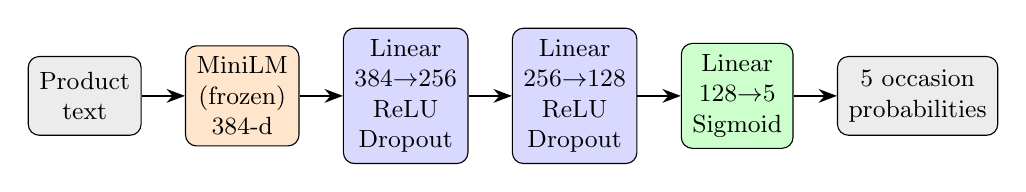
\begin{tikzpicture}[node distance=0.55cm, font=\small,
  box/.style={draw, rounded corners, minimum height=1.0cm, align=center, inner sep=4pt},
  arr/.style={-{Stealth}, thick}]
  \node[box, fill=gray!15] (txt) {Product\\text};
  \node[box, fill=orange!20, right=of txt] (enc) {MiniLM\\(frozen)\\384-d};
  \node[box, fill=blue!15, right=of enc] (l1) {Linear\\384$\to$256\\ReLU\\Dropout};
  \node[box, fill=blue!15, right=of l1] (l2) {Linear\\256$\to$128\\ReLU\\Dropout};
  \node[box, fill=green!20, right=of l2] (out) {Linear\\128$\to$5\\Sigmoid};
  \node[box, fill=gray!15, right=of out] (y) {5 occasion\\probabilities};
  \foreach \a/\b in {txt/enc, enc/l1, l1/l2, l2/out, out/y} \draw[arr] (\a) -- (\b);
\end{tikzpicture}
\caption{Architecture of the occasion classifier. Only the three linear layers are trained.}
\end{figure}

\begin{table}[htbp]
\centering
\small
\begin{tabular}{p{2.4cm}p{4.2cm}p{8.2cm}}
\toprule
Component & Choice & Reason \\
\midrule
Input & 384-d MiniLM sentence embedding & Captures meaning, not just keywords; small and fast on CPU \\
Hidden layers & 256 and 128 units, ReLU & Enough capacity for 5 labels with 17,476 training rows \\
Regularization & Dropout & Reduces co-adaptation; rate tuned (Table~\ref{tab:tuning}) \\
Output & 5 logits + sigmoid & Labels are not mutually exclusive, so independent probabilities are used instead of softmax \\
Loss & \texttt{BCEWithLogitsLoss} & Standard loss for multi-label targets; numerically stable \\
Optimizer & Adam & Adaptive step sizes; robust default for small MLPs \\
Threshold & 0.5 on each probability & Default; per-class tuning is future work \\
\bottomrule
\end{tabular}
\caption{Design decisions.}
\end{table}

\paragraph{Baseline.} To check that the neural network adds value, \texttt{baseline.py} trains a one-vs-rest \textbf{logistic regression} (\texttt{class\_weight=balanced}) on the same embeddings.

\paragraph{Preventing label leakage.} The occasion labels were derived from keyword rules applied to the same product text (Phase 2). The text field \texttt{text\_for\_embedding} contained the label string itself, so \texttt{make\_text()} removes this prefix and only the title and description are given to the model. Keywords in the title can still hint at the label; this is discussed in the limitations.

\subsection{Hyperparameter Tuning}
We ran a full grid search over \textbf{learning rate} $\in\{10^{-2},10^{-3},10^{-4}\}$, \textbf{batch size} $\in\{64,256\}$ and \textbf{dropout} $\in\{0.0,0.3\}$, giving \nConfigs\ configurations, each trained for 30 epochs with the Adam optimizer and seed 42. Configurations were ranked by macro F1 on the \emph{validation} set only; the test set was not touched during tuning.

\begin{table}[htbp]
\centering
\IfFileExists{tables/tuning.tex}{\begin{tabular}{lrrrrrr}
\toprule
LR & Batch & Dropout & Precision & Recall & F1 & AUC \\
\midrule
\textbf{0.001} & \textbf{64} & \textbf{0.3} & \textbf{0.933} & \textbf{0.918} & \textbf{0.925} & \textbf{0.978} \\
0.001 & 64 & 0 & 0.931 & 0.919 & 0.925 & 0.977 \\
0.001 & 256 & 0.3 & 0.923 & 0.925 & 0.924 & 0.977 \\
0.01 & 256 & 0 & 0.927 & 0.917 & 0.922 & 0.974 \\
0.001 & 256 & 0 & 0.923 & 0.920 & 0.922 & 0.977 \\
0.01 & 256 & 0.3 & 0.935 & 0.908 & 0.921 & 0.977 \\
0.01 & 64 & 0.3 & 0.931 & 0.910 & 0.920 & 0.976 \\
0.01 & 64 & 0 & 0.925 & 0.915 & 0.920 & 0.972 \\
0.0001 & 64 & 0 & 0.906 & 0.893 & 0.899 & 0.963 \\
0.0001 & 64 & 0.3 & 0.903 & 0.893 & 0.898 & 0.962 \\
0.0001 & 256 & 0 & 0.884 & 0.883 & 0.883 & 0.948 \\
0.0001 & 256 & 0.3 & 0.888 & 0.874 & 0.881 & 0.946 \\
\bottomrule
\end{tabular}
}{\textbf{[run src/plot\_results.py]}}
\caption{Hyperparameter search results on the validation set (best row in bold).}
\label{tab:tuning}
\end{table}

\safefig{tuning_f1}{Validation macro F1 for each configuration; the selected one is green.}

\paragraph{Final selection and justification.} The configuration with the highest validation macro F1 was selected: \textbf{learning rate \bestLR, batch size \bestBatch, dropout \bestDrop}, with validation macro F1 \bestValF\ and AUC-ROC \bestValAUC. We selected on F1 rather than accuracy because F1 balances precision and recall across the five labels, and we used the validation set so that the test set stays an unbiased final check. The results show that the \textbf{learning rate} has by far the largest effect: averaged over the other settings, $10^{-4}$ reached a validation F1 of only 0.890 because 30 epochs are too few for such small steps, while $10^{-3}$ (0.924) and $10^{-2}$ (0.921) were much better, and $10^{-3}$ scored slightly higher. A \textbf{batch size} of 64 was slightly better than 256 (0.915 versus 0.909), since smaller batches give more weight updates per epoch. \textbf{Dropout} made almost no difference (0.9117 without and 0.9115 with dropout on average), and the two best configurations differ by less than 0.001 F1. We kept dropout 0.3 because it was the top-ranked setting and, as Figure~\ref{fig:loss} shows, the network starts to overfit after about ten epochs, so a regularizer is a sensible safeguard even if its measured effect is small. Overall, the eight configurations with learning rate $10^{-3}$ or $10^{-2}$ lie within 0.006 F1 of each other, so the final result is not sensitive to the exact choice.
\section{Phase 4: Training \& Evaluation}

\subsection{Validation Strategy}
The cleaned dataset (24,967 products) was split once into \textbf{70\% train / 15\% validation / 15\% test} (17,476 / 3,745 / 3,746 products; \texttt{split\_data.py}), \textbf{stratified by product category} with a fixed seed (42), so that rare categories such as footwear and outerwear appear in every split. The training set fits the weights, the validation set is used for hyperparameter selection, and the test set (\testN\ products) is used \emph{once} for the final numbers. K-fold cross-validation was not used because the sentence embeddings are frozen and the dataset is large, so a single stratified hold-out gives stable estimates at a fraction of the cost.

\subsection{Training Behaviour}
\begin{figure}[htbp]
\centering
\IfFileExists{../figures/mlp_loss_curve.png}{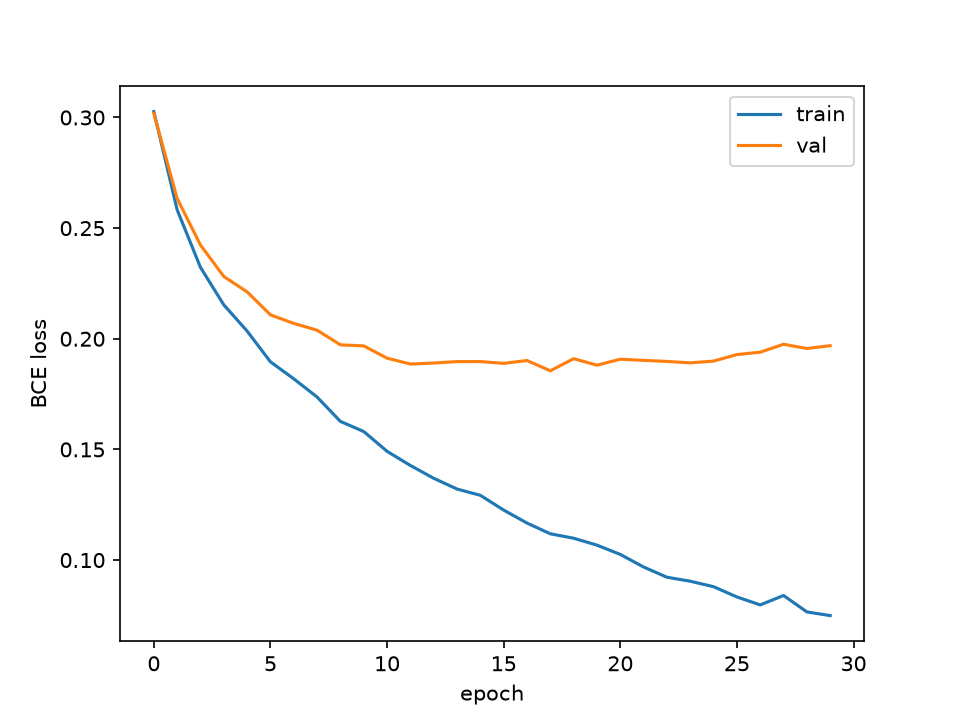
\includegraphics[width=0.7\linewidth]{../figures/mlp_loss_curve.png}}{\textbf{[missing]}}
\caption{Training and validation BCE loss of the selected model.}
\label{fig:loss}
\end{figure}
Figure~\ref{fig:loss} shows the binary cross-entropy loss per epoch. Both curves fall quickly from about 0.30 during the first ten epochs. The validation loss then flattens at about 0.19 and even rises slightly after epoch 25, while the training loss keeps decreasing to about 0.075. The growing gap shows that the network begins to overfit after roughly ten epochs. Since the weights of the last epoch are saved, early stopping (keeping the epoch with the lowest validation loss) would be a simple improvement; the gap is moderate and the test results below show that generalization is still good.

\subsection{Metrics and Why They Fit This Problem}
Plain accuracy is not informative for a multi-label task: each product has five yes/no decisions, and the labels are unevenly distributed (casual 68.7\%, presentation 53.9\%, office 53.8\%, concert 43.1\%, wedding 42.1\% of the test set), so a model leaning on the frequent labels would still score well on accuracy alone. We therefore report:
\begin{itemize}
  \item \textbf{Precision} -- of the products the model assigns to an occasion, how many truly belong. Low precision means the outfit builder would recommend unsuitable items.
  \item \textbf{Recall} -- of the products that suit an occasion, how many are found. Low recall shrinks the choice of items.
  \item \textbf{F1-score} -- harmonic mean of the two; we use the \emph{macro} average so rare occasions count as much as common ones.
  \item \textbf{AUC-ROC} -- threshold-independent ranking quality of the probabilities, useful because the 0.5 threshold is not tuned.
  \item \textbf{Exact match and Hamming loss} -- strict (all five labels right) and per-label error rates for the multi-label setting.
\end{itemize}

\subsection{Results on the Test Set}
\begin{table}[htbp]
\centering
\begin{tabular}{lcccc}
\toprule
Model & Precision & Recall & F1 & AUC-ROC \\
\midrule
Logistic regression (validation) & \baseP & \baseR & \baseF & \baseA \\
MLP, selected (validation) & 0.933 & 0.918 & \bestValF & \bestValAUC \\
\textbf{MLP, selected (test)} & \testPrec & \testRec & \testFone & \testAUC \\
\bottomrule
\end{tabular}
\caption{Macro-averaged metrics. Test micro-F1 is \testMicroF, Hamming loss \testHamming\ and exact-match ratio \testExact.}
\end{table}

The neural network clearly outperforms the logistic-regression baseline on the same validation data: macro F1 rises from \baseF\ to \bestValF\ and AUC-ROC from \baseA\ to \bestValAUC. The gain comes from both precision (0.896 against 0.933) and recall (\baseR\ against 0.918), so the non-linear hidden layers separate the occasions better than a linear model on the same embeddings. The test-set scores (F1 \testFone, AUC-ROC \testAUC) are about the same as the validation scores, so the model has not overfit the validation set through hyperparameter selection.

\begin{table}[htbp]
\centering
\IfFileExists{tables/per_class.tex}{\begin{tabular}{lrrrrrrrr}
\toprule
Class & Support & Prevalence & Precision & Recall & F1 & AUC & FP & FN \\
\midrule
casual & 2574 & 0.687 & 0.924 & 0.916 & 0.920 & 0.959 & 195 & 216 \\
concert & 1616 & 0.431 & 0.921 & 0.914 & 0.917 & 0.983 & 127 & 139 \\
office & 2014 & 0.538 & 0.940 & 0.938 & 0.939 & 0.985 & 120 & 125 \\
presentation & 2018 & 0.539 & 0.941 & 0.942 & 0.941 & 0.987 & 120 & 117 \\
wedding & 1577 & 0.421 & 0.940 & 0.906 & 0.923 & 0.983 & 91 & 148 \\
\bottomrule
\end{tabular}
}{\textbf{[run src/error\_analysis.py]}}
\caption{Per-class test results (FP/FN = false positives / false negatives).}
\label{tab:perclass}
\end{table}

\safefig{roc_per_class}{Per-class ROC curves on the test set.}

\subsection{Error Analysis}
\safefig{confusion_per_class}{Binary confusion matrix of each occasion label on the test set.}

Overall the model reaches a macro F1 of \testFone\ and an AUC-ROC of \testAUC\ on the test set, and 932 of the 3,746 test products (24.9\%) have at least one wrong label. The five classes perform very similarly (Table~\ref{tab:perclass}): F1 ranges only from 0.917 (concert) to 0.941 (presentation). Errors are balanced between false positives and false negatives. \emph{Casual} produces the most mistakes in absolute terms (195 false positives and 216 false negatives), partly because it is the most frequent label and has the lowest AUC (0.959); its definition is also the most vague, since it is the fallback label for products that match no other keyword rule. \emph{Wedding} has the lowest recall (0.906, 148 false negatives), which means some wedding products are missed, while its precision is high (0.940).

\emph{Office} and \emph{presentation} obtain the best scores (F1 0.939 and 0.941), but this should not be read as a deeper understanding of formal wear. As noted in Phase 2, these two labels come from almost identical keyword lists, so they are nearly the same label, and in interactive tests the model predicted them together (for example, ``formal blazer'' scored 1.00 for both). The very high scores also reflect that the labels are derived by keyword rules from the same product text: the network mainly learns to reproduce those rules, so some of the remaining errors are caused by noisy labels (for example ``blazer'' was also predicted as casual with probability 0.90) rather than by the model.

Table~\ref{tab:errors} lists the most confident mistakes. Many involve products whose title contains a keyword that conflicts with the description, or labels produced by broad keyword rules (e.g.\ ``embroidered'' $\to$ wedding), which means part of the ``error'' is noise in the heuristic labels rather than a model failure.
\begin{table}[htbp]
\centering
\small
\IfFileExists{tables/errors.tex}{\begin{tabular}{p{4.6cm}p{2.2cm}p{3cm}p{3cm}}
\toprule
Product title & Brand & True labels & Predicted \\
\midrule
EARRINGS (E2840/111/131) & Ethnc & concert & casual|office|presentation \\
CHUNKY SLIDES & Lama & concert & casual|concert \\
White Cotton Shalwar (MPS25SH1W004) & Bonanza Satr & casual|wedding & casual \\
Regil Long & Lulusar & casual & casual|concert|office|presentation \\
SHIRT (E0750/119/112) & Ethnc & wedding & office|presentation|wedding \\
SKIRT (E3602/108/901) & Ethnc & office|presentation & office|presentation|wedding \\
Bella - 3 PC (WSS25P3024) & Bonanza Satr & concert|office|presentation|wedding & casual|concert|office|presentation \\
BROWN TRENDY PESHAWARI SANDALS & J. & casual|wedding & casual \\
\bottomrule
\end{tabular}
}{\textbf{[run src/error\_analysis.py]}}
\caption{Most confident errors on the test set.}
\label{tab:errors}
\end{table}

\subsection{Bias Check}
The project aims at inclusive recommendations, so we checked whether performance differs across groups. Skin-tone and body-type labels do not exist in the data yet (Phase 2), so \textbf{brand, gender, category and plus-size availability} are used as available proxies: if the model works much worse for a group, products from that group (e.g.\ women's wear, plus-size items, small brands) would receive worse recommendations.

\safefig{bias_check}{Macro F1 per subgroup on the test set (groups with fewer than 30 products are skipped).}
\begin{table}[htbp]
\centering
\small
\IfFileExists{tables/bias.tex}{\begin{tabular}{llrrr}
\toprule
Attribute & Group & n & Macro F1 & Gap vs overall \\
\midrule
brand & Lama & 68 & 0.695 & -0.233 \\
brand & Lulusar & 407 & 0.765 & -0.163 \\
brand & Ethnc & 446 & 0.867 & -0.061 \\
brand & Hussain Rehar & 36 & 0.928 & -0.000 \\
brand & J. & 1255 & 0.953 & 0.025 \\
brand & Bonanza Satrangi & 1356 & 0.956 & 0.028 \\
brand & Outfitters & 149 & 0.971 & 0.043 \\
category & top & 764 & 0.855 & -0.073 \\
category & accessory & 345 & 0.860 & -0.068 \\
category & footwear & 119 & 0.875 & -0.053 \\
category & bottom & 538 & 0.878 & -0.050 \\
category & outerwear & 77 & 0.893 & -0.035 \\
category & set & 1903 & 0.957 & 0.029 \\
gender & unisex & 771 & 0.879 & -0.049 \\
gender & women & 2130 & 0.943 & 0.015 \\
gender & men & 845 & 0.950 & 0.022 \\
has\_plus\_sizes & 1 & 677 & 0.919 & -0.009 \\
has\_plus\_sizes & 0 & 3069 & 0.930 & 0.002 \\
\bottomrule
\end{tabular}
}{\textbf{[run src/plot\_results.py]}}
\caption{Subgroup macro F1 and gap to the overall test F1.}
\end{table}

Overall test macro F1 is \testFone. Performance is very similar for plus-size and other products (0.919 for products offering 2XL or larger, 0.930 for the rest, a gap of 0.011), so we found no meaningful disadvantage for plus-size items. Gender differences are small for men (0.950) and women (0.943), but \emph{unisex} products score lower (0.879).

The largest differences appear across \textbf{brands} and \textbf{categories}. Among brands, F1 ranges from 0.971 (Outfitters) and 0.956 (Bonanza Satrangi) down to 0.867 (Ethnc), 0.765 (Lulusar) and 0.695 (Lama), a spread of 0.276. Lama has only 68 test products, so its estimate is noisy, but Lulusar (407 products) is a reliable signal that the model is clearly worse on this brand, 0.163 below the overall score. Among categories, sets score highest (0.957) while tops (0.855), accessories (0.860) and bottoms (0.878) are 5 to 7 points below the average. A likely reason is that the dataset is dominated by a few brands and by sets (50.8\% of all products), so the model sees much more of their vocabulary and style of description, while other brands and single garments use different wording; we did not test this explanation directly. In the final application, recommendations for the weaker brands and categories (and for unisex items) would therefore be less reliable, so the occasion check should be treated with more caution for them. Possible remedies are oversampling weak groups, brand-balanced training and evaluation, and manual label checks on the weak subgroups.

\paragraph{Limitations.} (i) The labels are keyword heuristics derived from the same text the model reads, so high scores partly measure how well the network reproduces our rules, not real shopper opinion; (ii) the data comes from two dominant brands (68.7\% of products); (iii) no real demographic attributes are available, so the bias check cannot assess skin tone or body type directly; (iv) the threshold of 0.5 is the same for all labels; (v) the final epoch rather than the best epoch is saved. Future work: manual labels for a sample, per-class thresholds, early stopping, and fine-tuning the encoder.
\section{Phase 5: Output Execution (Track A: Application)}

We integrated the trained model into a Streamlit web application \cite{streamlit}. The source code is available at
\url{https://github.com/Romeshaafzaal/Trouvaille}, and the app is run locally with \texttt{python -m streamlit run app.py}
(see the \texttt{README.md} for setup).

\subsection{Model Used in the App}
The application uses the occasion classifier from Phase 3: a PyTorch MLP \cite{paszke2019pytorch} trained with the Adam optimizer \cite{kingma2015adam}
on 384-dimensional sentence embeddings of product text \cite{reimers2019sbert,wang2020minilm}. A scikit-learn \cite{pedregosa2011sklearn}
logistic regression on the same embeddings served as the baseline (validation macro F1 0.878). The selected MLP (learning rate $10^{-3}$, batch size 64, dropout 0.3)
reaches a test macro F1 of 0.928 and an AUC-ROC of 0.980. To keep the interface fast, the MLP is run once over the whole catalogue offline
(\texttt{src/prepare\_app\_data.py}), and the resulting occasion probabilities are stored next to each product in \texttt{app\_data/products\_app.csv}.

\subsection{System Architecture}
\begin{figure}[!htbp]\centering
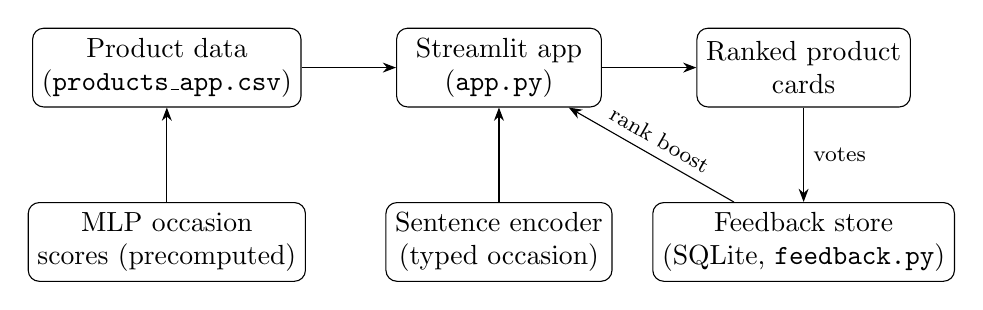
\begin{tikzpicture}[node distance=1.2cm, box/.style={draw, rounded corners, align=center, minimum width=2.6cm, minimum height=1cm}, >=Stealth]
  \node[box] (data) {Product data\\(\texttt{products\_app.csv})};
  \node[box, right=of data] (app) {Streamlit app\\(\texttt{app.py})};
  \node[box, right=of app] (out) {Ranked product\\cards};
  \node[box, below=of data] (mlp) {MLP occasion\\scores (precomputed)};
  \node[box, below=of app] (enc) {Sentence encoder\\(typed occasion)};
  \node[box, below=of out] (fb) {Feedback store\\(SQLite, \texttt{feedback.py})};
  \draw[->] (mlp) -- (data);
  \draw[->] (data) -- (app);
  \draw[->] (enc) -- (app);
  \draw[->] (app) -- (out);
  \draw[->] (out) -- node[right, font=\footnotesize]{votes} (fb);
  \draw[->] (fb) -- node[above, sloped, font=\footnotesize]{rank boost} (app);
\end{tikzpicture}
\caption{Application architecture. The trained MLP scores every product once offline; at request time the app matches the typed occasion, filters the catalogue and ranks by the occasion score. Thumbs up/down votes are stored in a local SQLite file and feed back into the ranking as a small capped adjustment.}
\end{figure}

\subsection{Features}
\begin{itemize}
  \item \textbf{Occasion input:} the user chooses one of five occasions (wedding, office, presentation, concert, casual) or types any text. Typed text is embedded with the same sentence encoder and matched to the closest occasion by cosine similarity; if the similarity is below 0.25 the app asks the user to rephrase.
  \item \textbf{Budget:} minimum and maximum price are typed in and validated (whole numbers, minimum not above maximum, sanity limit).
  \item \textbf{Filters:} gender, product type, color, size, skin undertone, body type and in-stock only. Size and body type apply to clothing only, so footwear and accessories are not removed by them.
  \item \textbf{Ranking and display:} products with an occasion probability of at least 0.5 are kept. Their rank is the occasion probability, plus $0.4\times$ a colour score when a skin undertone is chosen, plus $0.4\times$ a fit score when a body type is chosen, plus a small feedback adjustment (below). Products are shown as cards (image, brand, price, discount, match percentage and a link to the store) with pagination, and the page resets to the first page whenever a filter changes.
  \item \textbf{Feedback:} each card has thumbs-up and thumbs-down buttons. Every vote is stored with the product, the occasion and a timestamp in a local SQLite database. A product's rank is adjusted by $0.2\,(u-d)/(u+d+5)$, where $u$ and $d$ are its up and down votes for that occasion, so the adjustment stays within $\pm0.2$ and needs several votes to matter. A ``Community feedback'' panel shows the approval rate per occasion and the most and least liked products.
  \item \textbf{Saved outfits:} a heart button on each card saves the outfit to a sidebar list with a link to the store, a remove button and a CSV download. The list is kept in the browser session only.
\end{itemize}

\subsection{Learned and Rule-Based Components}
Two parts of the system are learned: the occasion classifier (an MLP trained on our data) and the semantic matching of typed occasions (a pretrained encoder).
Everything else is rule-based. Skin undertone matching uses a color-to-undertone lookup inspired by seasonal color analysis \cite{jackson1980color}, applied when the data was cleaned.
Body type is approximated from fit keywords (fitted, regular, relaxed), and from plus-size availability and stretch for the curvy option.
Budget, color, size and gender use catalogue fields directly. These rule-based parts are heuristics and were not evaluated against human judgements.

\subsection{Application Screenshots}
\IfFileExists{../figures/app_results.png}{%
\begin{figure}[htbp]\centering
  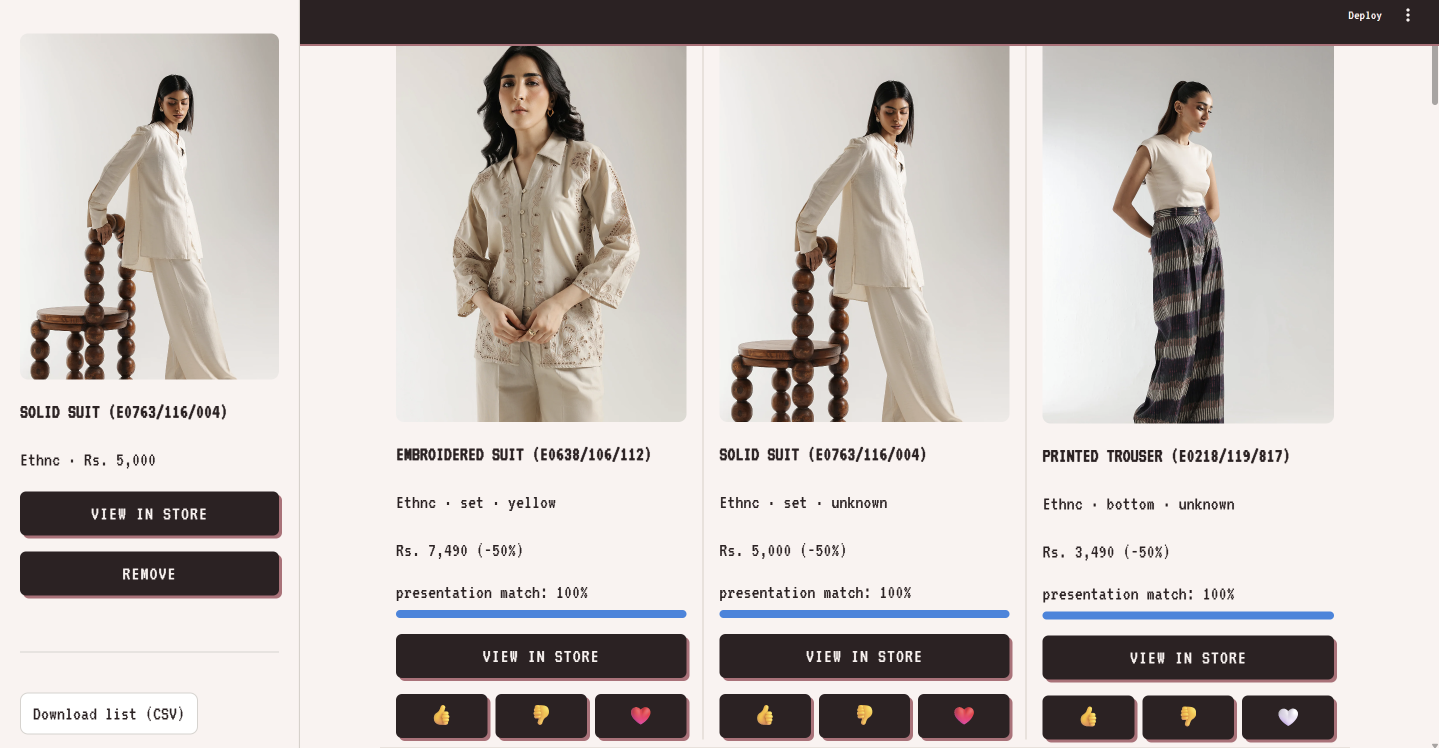
\includegraphics[width=\linewidth]{../figures/app_results.png}
  \caption{Results page for the occasion ``presentation'' with no colour filter. Each card has a store link and thumbs-up, thumbs-down and save buttons; the sidebar on the left shows a saved outfit with its remove button and the CSV download.}
\end{figure}}{\textbf{[Missing figure: app\_results.png]}\par}

\IfFileExists{../figures/app_filters.png}{%
\begin{figure}[htbp]\centering
  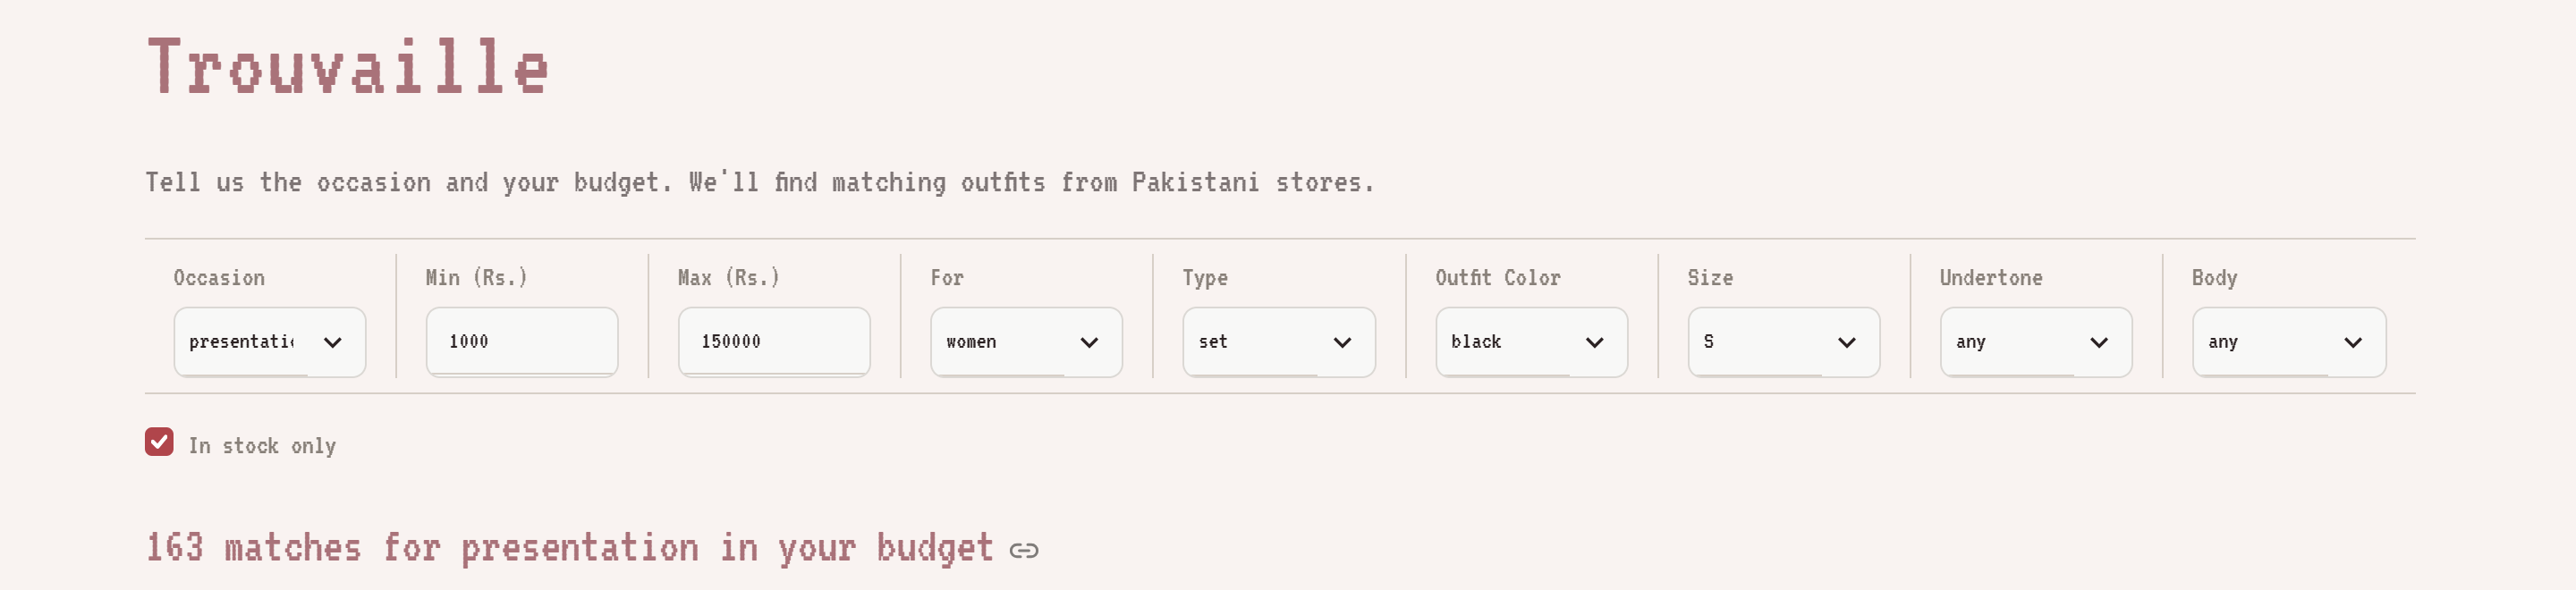
\includegraphics[width=\linewidth]{../figures/app_filters.png}
  \caption{The filter bar: occasion, minimum and maximum price, gender, type, outfit colour, size, undertone and body type, plus the in-stock checkbox. The line below it reports the number of matches (163 here).}
\end{figure}}{\textbf{[Missing figure: app\_filters.png]}\par}

\subsection{Sample Predictions}
Table~\ref{tab:samples} shows five searches run on the app's data (in stock only, probability of at least 0.5). The similarity is the cosine similarity between the typed text and the matched occasion.

\begin{table}[htbp]\centering\small
\begin{tabular}{p{2.6cm} p{2.5cm} p{1.5cm} p{5.6cm}}
\toprule
Search (budget) & Matched occasion (similarity) & Matches & Top result \\
\midrule
``graduation'' (Rs.~15{,}000) & presentation (0.52) & 4{,}332 & Ethnc, Printed Trouser, Rs.~3{,}490 \\
``wedding'' (Rs.~15{,}000) & wedding (0.59) & 4{,}167 & Outfitters, Relaxed Fit Washed Out Trousers, Rs.~4{,}890 \\
``office'', size M (Rs.~8{,}000) & office (0.60) & 2{,}352 & Ethnc, Printed Trouser, Rs.~3{,}490 \\
``party'' (Rs.~10{,}000) & concert (0.54) & 3{,}387 & J., Cream Lawn Digital Printed Unstitched 2Pc, Rs.~3{,}490 \\
``lehenga'' (Rs.~15{,}000) & wedding (0.14) & 4{,}167 & Rejected by the app (below the 0.25 cutoff) \\
\bottomrule
\end{tabular}
\caption{Sample searches. Counts are for the whole catalogue with no gender, type, color or other filters.}
\label{tab:samples}
\end{table}

The text matching behaves sensibly for phrases the model was not trained on: ``graduation'' maps to presentation and ``party'' to concert.
However, the ranking itself is weak. The top results often show a probability of about 100\%, so many products tie at the top and their order is not informative,
and some top results are hard to justify, such as washed-out trousers for a wedding.

\subsection{Result Discussion}
\paragraph{Why samples fail.} The occasion labels were produced by keyword rules, so the classifier largely learns to reproduce them; its high test score (macro F1 0.928) measures agreement with those rules, not with how a human would judge an outfit.
The model is also multi-label and gives high probabilities to several occasions for many products, which produces the ties and implausible top results seen above.
We did not investigate the cause further; noisy keyword labels are the most likely explanation, and hand-labelled data would be needed to confirm it.

\paragraph{Subgroup weaknesses.} The bias check on the test set showed lower macro F1 for some brands (Lama 0.695 on 68 items, Lulusar 0.765, Ethnc 0.867) than for others (Outfitters 0.971, Bonanza Satrangi 0.956),
and for some categories (tops 0.855, accessories 0.860, bottoms 0.878) than for sets (0.957). Unisex items (0.879) scored below men's (0.950) and women's (0.943) items.
A plausible reason is that these brands and categories describe products differently, so the keyword rules fit them less well, but we did not test this.

\paragraph{The ``lehenga'' query.} Searching for ``lehenga'' returned no results. The catalogue contains no product with ``lehenga'' in its title, and the query's similarity to the closest occasion (0.14) is below the app's cutoff, so the app asks the user to rephrase.
This is consistent with the data limitation that the luxury and bridal segment is almost absent from the scraped brands.

\subsection{Limitations and Future Work}
\begin{itemize}
  \item The app is run locally and is not hosted online.
  \item The size filter shows products that offer a size, not whether that size is in stock, because the scraped data holds only a product-level availability flag.
  \item Occasion labels, undertone matching and body-type filtering are heuristics. There is no learned skin-tone or body-type model, and no product ratings were collected. The thumbs-up/down feedback is stored in a local file, was only tried with a handful of test votes, and has not been evaluated; on a hosted deployment it would need persistent storage.
  \item The original project goal also included LLM query parsing, ratings-based re-ranking, an outfit builder and a Vibe Check Engine. These are not implemented; the app filters and ranks single products.
  \item Ranking is coarse: many products tie near 100\%, and results are not personalised. The feedback adjustment is capped at $\pm0.2$, so it only reorders products that are already close in score. The saved-outfits list is lost when the page is refreshed.
  \item The data is a single snapshot from eight effective brands, taken during a sale period, and kids' wear, luxury and bridal wear are largely missing.
  \item Future work: hosting the app online, hand-labelled evaluation data, per-variant stock scraping, a calibrated or fine-tuned model that separates occasions better, and learned undertone suitability.
\end{itemize}
\section{Team Contributions \& Version Control}
All code was committed with the Git command line, working on feature branches and merging them into \texttt{main}. The first table is generated automatically from the repository history by \texttt{src/contrib\_table.py} and lists every commit made for Deliverable 3 together with the files it changed. The second table summarises who wrote which module.

{\small
\IfFileExists{tables/contributions.tex}{\begin{longtable}{p{2.6cm}p{1.3cm}p{4.4cm}p{6.2cm}}
\caption{Git commits for Deliverable 3 (generated by \texttt{src/contrib\_table.py}).}\\
\toprule
Author & Commit & Files / module & Message \\
\midrule
\endfirsthead
\toprule
Author & Commit & Files / module & Message \\
\midrule
\endhead
\bottomrule
\endfoot
Romesha Afzaal & \texttt{9626508} & app\_data/products\_app.csv, src/prepare\_app\_data.py & Prepare app data with occasion scores \\
Romesha Afzaal & \texttt{fa8f64b} & app.py & Add Streamlit app with validated budget inputs \\
Romesha Afzaal & \texttt{74929bd} & app.py & Add outfit color filter \\
Romesha Afzaal & \texttt{0b12312} & app.py, app\_data/products\_app.csv, src/prepare\_app\_data.py & Add size filter and extra app columns \\
Romesha Afzaal & \texttt{7ac6688} & app.py & Add body type filter \\
Romesha Afzaal & \texttt{3f40ff3} & app.py & Add app filters \\
Romesha Afzaal & \texttt{1bb4b16} & app.py, style.css & Add app filters and styling \\
Romesha Afzaal & \texttt{5c27ee2} & app.py & Add pagination with scroll to top \\
Romesha Afzaal & \texttt{205b824} & app.py & Skip size and body type filters for footwear and accessories \\
Romesha Afzaal & \texttt{779f47a} & app.py & change the filters layout \\
Romesha Afzaal & \texttt{db4e5d7} & app.py & improve the occasion detection \\
Romesha Afzaal & \texttt{1f579e4} & app.py, style.css & improve the filters interface \\
Romesha Afzaal & \texttt{8fdbbe0} & app.py & use -+ buttons for pagination \\
Romesha Afzaal & \texttt{2ebba89} & app.py & Add loading splash screen \\
Romesha Afzaal & \texttt{61cfecf} & app.py & Fix scroll to top on page change \\
Romesha Afzaal & \texttt{a386827} & app.py & Remove duplicate occasion matcher \\
Romesha Afzaal & \texttt{fccc130} & app.py & Replace undertone hard filter with color-based ranking \\
Romesha Afzaal & \texttt{483cede} & app.py & Add body fit scoring and fix tone/fit float casting \\
Romesha Afzaal & \texttt{51bc837} & app.py & Reset pagination to page 1 when filters change \\
Romesha Afzaal & \texttt{7492d66} & requirements.txt & Change requirements.txt for deliverable 3 \\
Romesha Afzaal & \texttt{a19bf8a} & README.md & Revise README to enhance project clarity \\
Romesha Afzaal & \texttt{2aed6a5} & README.md & Document Deliverable 3: Application and its features \\
Romesha Afzaal & \texttt{a5ce384} & README.md & Update README with new repository structure details \\
Romesha Afzaal & \texttt{757f105} & README.md & Add app screenshot \\
Romesha Afzaal & \texttt{18c88da} & README.md & Revise image formatting and add results page header \\
Romesha Afzaal & \texttt{3d69991} & app.py & Add the dropdown with the textField for occasion \\
Romesha Afzaal & \texttt{c828d17} & (none) & Add dropdown with the textBox in the occasion field \\
Aliza Nadeem & \texttt{48fcb7a} & feedback.py & Add SQLite feedback storage module \\
Aliza Nadeem & \texttt{92e3a3c} & app.py & Add thumbs up/down feedback buttons to result cards \\
Aliza Nadeem & \texttt{fe8a6f2} & style.css & Fix feedback button label clipping \\
Aliza Nadeem & \texttt{7eb00ac} & style.css & Use uniform 3:4 product image frames \\
Aliza Nadeem & \texttt{ca7f205} & app.py & Adjust ranking using community feedback (capped boost) \\
Aliza Nadeem & \texttt{d7e22d3} & app.py & Add community feedback insights section \\
Aliza Nadeem & \texttt{afe85a4} & README.md & Document feedback feature in README \\
Aliza Nadeem & \texttt{9b69af4} & (none) & Merge pull request \#4 from Romeshaafzaal/feature/user-feedback \\
Aliza Nadeem & \texttt{8a1f198} & app.py & Add save-to-favorites heart button on result cards \\
Aliza Nadeem & \texttt{504eeed} & app.py & Add saved outfits sidebar with remove and CSV export \\
Aliza Nadeem & \texttt{14d0527} & README.md & Document saved outfits feature in README \\
Aliza Nadeem & \texttt{4b3d060} & style.css & Style save button and saved outfits sidebar \\
Aliza Nadeem & \texttt{4e18d65} & (none) & Merge branch 'feature/saved-outfits': add saved outfits \\
Aliza Nadeem & \texttt{856295f} & .gitignore & Ignore local feedback database \\
Aliza Nadeem & \texttt{2a05f96} & app.py, style.css & Use compact emoji action row on result cards \\
Aliza Nadeem & \texttt{0a4eedd} & (none) & Merge branch 'feature/emoji-buttons': compact emoji action row \\
Aliza Nadeem & \texttt{d6e93fe} & src/contrib\_table.py & Generate contribution table as multi-page longtable \\
Aliza Nadeem & \texttt{d081698} & report/contributions.tex, report/main.tex, report/phase5.tex, report/references.bib & Add Deliverable 3 report source: application, feedback and saved outfits \\
Aliza Nadeem & \texttt{306c069} & (none) & Add application screenshots for the report \\
\end{longtable}
}{\textbf{[run src/contrib\_table.py]}}
}

\begin{table}[htbp]
\centering
\small
\begin{tabular}{p{3cm}p{10.5cm}}
\toprule
Member & Deliverable 3 modules \\
\midrule
Romesha Afzaal & \texttt{src/prepare\_app\_data.py} (precomputes occasion scores), \texttt{app.py} (budget validation, occasion matching, filters, undertone and body-type scoring, pagination, loading screen), \texttt{style.css} (interface styling), \texttt{requirements.txt}, application README \\
Aliza Nadeem & \texttt{feedback.py} (SQLite feedback storage and ranking adjustment), thumbs-up/down buttons and the community feedback panel, saved outfits sidebar with CSV export, compact action row and card styling in \texttt{app.py} and \texttt{style.css}, README sections for both features \\
\bottomrule
\end{tabular}
\caption{Module ownership for Deliverable 3. Deliverable 2 ownership is in the Deliverable 2 report.}
\end{table}

\paragraph{Model weights.} Trained weights (\texttt{mlp\_occasion.pt}) are hosted on Google Drive; the link is in \texttt{README.md}. Code: \url{https://github.com/Romeshaafzaal/Trouvaille}.


\bibliographystyle{plain}
\bibliography{references}

\end{document}